\chapter{Designing and Building the System} \label{HLFHealthcare}  

The goal of this thesis is to evaluate the suitability of Blockchain technology
in managing the identity of patients in an Healthcare organization by
conceptualizing and implementing a system that fulfills this role. In order to
fulfill this goal, the development part of this thesis was primarily divided
into four steps with each step building upon the previous ones. This Chapter
provides an insight into how the desired functionality was achieved by the
system starting at the conceptualization and its associated challenges all the
way to the implementation of said system. This system was built using some of
the technologies and concepts described in the previous section.

\section{First Step - Defining Requirements and Choosing a 
	Platform}\label{choosingHyperledger}

After investigating the various Blockchain platforms some criteria was needed
to serve as reference. As such, the first step consisted in defining a set of
key points that the built system had to fulfill. Defining the requirements
proved helpful to choose the most appropriate platform for the objectives as
explained later.

\subsection{Requirement Definition}
The requirements for this project were deemed to be as follows:

\renewcommand{\labelenumi}{\Roman{enumi}.}
\begin{enumerate}
  \item The system must allow a patient to opt into the network and register as
    a participant.
  \item The system must allow a patient to record his medical data under the
    approval of an administrator.
  \item The system must keep information confidential, transparent and have
    high availability.
  \item The system must provide the patient with the ability to share his data
    with another entity participating in the network, for example sharing
    information with a doctor.
  \item The system must allow the deletion of a patient's data in some manner,
    if he wishes to do so, in order to comply with European privacy laws.
\end{enumerate}

These requirements were chosen in order to create a system that is interesting
to an organization while still respecting the patients data and their access
right to it. 

After defining the requirements it was nececessary to choose the Blockchain
platform that best fulfills these requirements.


\subsection{Choosing a Platform}\label{choosePlatform}

Blockchain platforms often have different goals even tough they normally
originate from the realization that full centralization has major drawbacks.
Ranging from open networks, such as Ethereum which anyone can join and use, to
permissioned distributed ledgers, which can be run publicly or privately but
are only open to access and participation through a membership service, such as
Hyperledger Fabric and Hyperledger Indy.

Ethereum is a popular platform on its own right and has certainly paved the way
for Blockchain to be used as a platform that can be extended and built upon. It
has a growing learning ecosystem and community. It is easy to start interacting
with the network as anyone is able to simply download a client and connect to
it.  Thanks to the Solidity smart contract language being targeted for the
specific purpose of authoring smart contracts it is a platform easy to develop
for after the initial learning barrier of the \textbf{dsl}. 

Ethereum is being used in a great deal of projects around the world proving its
stability and suitability in a wide variety of use cases. On the other hand,
handling patients medical data is a great responsibility due to the private and
personal nature of this data. Also hospitals and clinics must obey the
regulatory laws regarding privacy and usage of this data.

It is also worth noting that while Ethereum can handle private data exchange by
building upon it, as shown by Barclay, it was not designed with this intent in
mind, therefore these middle ground solutions can prove to be unwise to use at
scale given Ethereum's and the whole Blockchain's ecosystem past problems with
scalability.  

Fabric, like Ethereum, was built with the intention of being a general purpose
use Blockchain. It provides developers with the tools needed to build any
system they can imagine. However, the latter is clearly focused on making
organizations feel more at ease by being auditable as it offers an identity
service and a known environment due to using a membership service provider and
a certificate authority, therefore avoiding the same fate as \textbf{IoT}
devices where the lack of security regulations and ambiguity in how data
collected by these devices is handled has stopped these to be used in any
official capacity.

Fabric also has good amount of development tools that are now maturing and a
good learning environment with ample documentation about every aspect important
for a developer looking to get started into it. Fabric is being backed by the
Linux Foundation and IBM, lending credibility to the project and ensuring that
this platform is supported and developed in the foreseeable future, being
governed by a diverse technical steering committee and by a diverse set of
maintainers from multiple organizations. In regards to performance the
Hyperledger community is appointed a Performance and Scale working group to
improve performance as well as implementation of a benchmarking framework
called Hyperledger Caliper.

Regarding Fabric's features, it lends itself very well to fulfill the project
requirements. With Fabric's channels and private data segregation at peer level
it lends itself well to fulfill all the requirements that were laid out for
this project. Adding to this, many Blockchain based projects in the Healthcare
field are using permissioned networks due to the concerns regarding the privacy
of the patients while retaining the key benefits of Blockchain such as
immutability and decentralization.

Ultimately it was decided to use Hyperledger Fabric as the platform on which to
build the prototype project upon.


\section{Working knowledge of the Platform}

After choosing to work with Hyperledger Fabric it became necessary to
understand in further detail what are the components that form a network and
the tools to manage these components. This section discusses the main
components of a Fabric network and the tools required to create and maintain a
Fabric network. These components often interact with one another and provide
the technical infrastructure that comprises this technology. This knowledge
proved essential in building the solution proposed by this Thesis.

\subsection{Hyperledger Fabric Components}

An Hyperledger Fabric (HLF) network is defined as the technical infrastructure
that provides ledger and smart contract services to applications. Smart
contracts are used to generate transactions and interact with the ledger. The
network is comprised of several components. 

The ledger is one of these components, composed by a world state and a
Blockchain. The world state is a database that holds the current values of
ledger states. States are, by default, expressed as key-value pairs. The world
state is useful because it makes it easy for a program to get the current value
of these states, instead of having to traverse the entire transaction log. The
Blockchain holds the transaction logs that record the history of changes that
have resulted in the current world state. Transactions are collected and
recorded in an immutable sequence of blocks. Each block contains a set of
ordered transactions. There is one logical ledger in a Hyperledger Fabric
network, even tough in reality, the network maintains multiple copies of a
ledger that are synchronized through consensus. 

Another component is the set of peers participating in the network. A Peer is a
node that hosts a copy of the multiple ledgers and smart contracts. HLF opts to
allow multiple ledgers in a network to achieve different goals of a greater
purpose. This allows the creation of channels of information between trusted
parties, for example, a channel of secure and private information between the
clinical staff of an hospital and a patient as discussed on
Chapter~\ref{background}. 

Through a peer connection, applications execute chaincode that queries or
updates a ledger. Peers have at least one of the three different roles assigned
to them, as seen on Section~\ref{distributedLedgerPlatform}. Applications
always connect to peers when they need to access ledgers and smart contracts.
Every peer in the network is assigned a digital certificate by an administrator
from its owning organization. The mapping of a peer's identity in an
organization is provided through the membership service provider. 

In fact peers, applications, end users (clients), administrators, channels and
organizations must have an identity provided by the MSP in order to be able to
interact with the network. Each of these actors has a digital identity
encapsulated in an X.509 digital certificate standard. These determine the
exact permissions these have over resources and access to information in the
network. The MSP issues these certificates through the built-in CA component,
the Fabric Certificate Authority (CA). The Fabric CA is a private root CA
provider that consists in a CA server and a CA client. The MSP also supports
Certificate Revocation Lists (CRL).

\subsection{Administrating a HLF Networks}


As discussed, a HLF network must have an administrator. HLF provides the
\textit{cryptogen}, \textit{configtxgen}, \textit{configtxlator} and
\textit{peer} tools that are used to configure the network to suit different
needs and use cases.

The \textit{cryptogen} tool generates cryptographic data consuming the file
\textit{crypto-config.yaml}.  HLF uses an abstraction layer for certification
and authority called Membership Service Provider (MSP) that defines the rules
by which entities are governed and authenticated and it must be unique for
every participating entity.

The \textit{configtxgen} tool generates the genesis block for the orderer
services and the initial transactions.  This tool consumes the file
\textit{configtx.yaml} that defines configuration parameters for channels, the
genesis block and the orderer service.

The \textit{configtxlator} tool is also used to generate channel
configurations.  Finally the \textit{peer} tool is used to manage the
participating peers in the HLF network.

These tools are used to create and maintain the topology of the network and are
invoked when a change to the network is made, for example, when permissions to
certain records are changed or a new user is enrolled in the network and are
very much intertwined with the Fabric Certificate Authority (CA) discussed in
subsection .

\section{Building the System}

After considering the project goals of investigating the suitability of a
Blockchain based system to manage patients in Healthcare, the third step was to
build a prototype of a system that would represent the network, albeit on a
smaller scale. The insights gained from developing a simple working system
would enable benefits and risks of the approach to be identified, and
opportunities for further research to be laid out.

\subsection{Designing the System}

In order to build a system it is a good practice to conceptualize the
architecture first. After some consideration the concept was determined to be
as follows:

The information that defines the patients identity is a key requirement to
build a system that recognizes patients across the Healthcare environment, as
discussed in Chapter~\ref{background}. An asset can be created that represents
the concept of the patient's identity in this network.

To aid in interoperability with other systems, as seen in Figure
\ref{fig:interoperability}, the Fast Healthcare Interoperability Resources
(FHIR) standard by the Health Level 7 organization was used as basis for the
representation of a patient.  Each field of the structure that represents the
patients identity, defined in the smart contract, is linked to a field of the
\href{http://www.hl7.org/fhir/patient.html}{patient structure as presented in
the FHIR standard}.

\begin{figure}[ht] \centering
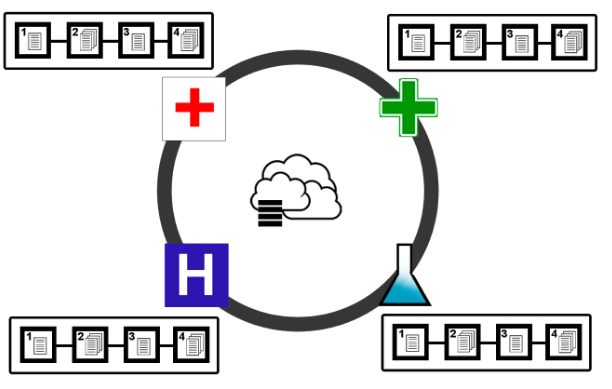
\includegraphics[width=0.7\linewidth]{imgs/interoperability.png}
\caption{\label{fig:interoperability}An Example of Interoperability with the
Blockchain Network} \end{figure}

% Falar sobre channels, organizations, peers, permissões. Falar sobre 
% precupações dúvidas, dificuldades, objectivos.

The most simple case of an interaction in an Healthcare service is the
interaction between a patient and a doctor. In HLF this situation translates to
two organizations and two peers. Each peer belongs to an organization. One
organization represents the patients while the other represents the hospital
where the doctor works. 

To establish a communication between the two participating peers a channel can
be created ensuring information exchanged between the two on the channel is
private and does not exist on the rest of the network.  If a third organization
with another peer representing another health clinic joined the network then
another channel could be created between the patient's organization and this
new organization. If the patient were to insert his data into the channel then
the clinic would be able to view it everytime they wished. 

Starting in version 1.1 of Fabric the MSP allows Attribute Based Access Control
meaning access flow to the data can depend on the value of a certain attribute
of the certificate. Also it is possible to encrypt data and insert it into the
channel and then require a key to decrypt the data. In this case the patient
could give a key to the doctor to be able to access only his data. In the
current version of Fabric, version 1.2, private data collections was
introduced, meaning that some data can be marked as private on a channel while
other data can be public.


\subsection{Creating the System}

To create an interactive system that can manage the patients identity in an
Healthcare environment an application was built that the user interacts with.
This application interfaces with smart contracts through the Hyperledger Fabric
Software Development Kit and the chaincode was built using the Hyperledger
Fabric Shim for node.js.

The identity of a patient was recorded on the ledger of the HLF network as a
structure via chaincode deployed to the network that interacts directly with
the ledger.  This structure contains the necessary fields to identify the
patient such as its name and birth date, for example, as well as some other
information necessary to manage this data. 

The application is accessed by the user and calls upon the smart contract.  The
smart contract will handle the assets part of the system.  A smart contract to
represent and manipulate identity was built and interfaces with the network to
write and read records to the appropriate ledger. The overview of the
architecture for this system is represented on Figure \ref{fig:appOverview}.
The smart contract also initializes and manages the ledger state through
transactions as well as the world state.

\begin{figure}[ht] \centering
  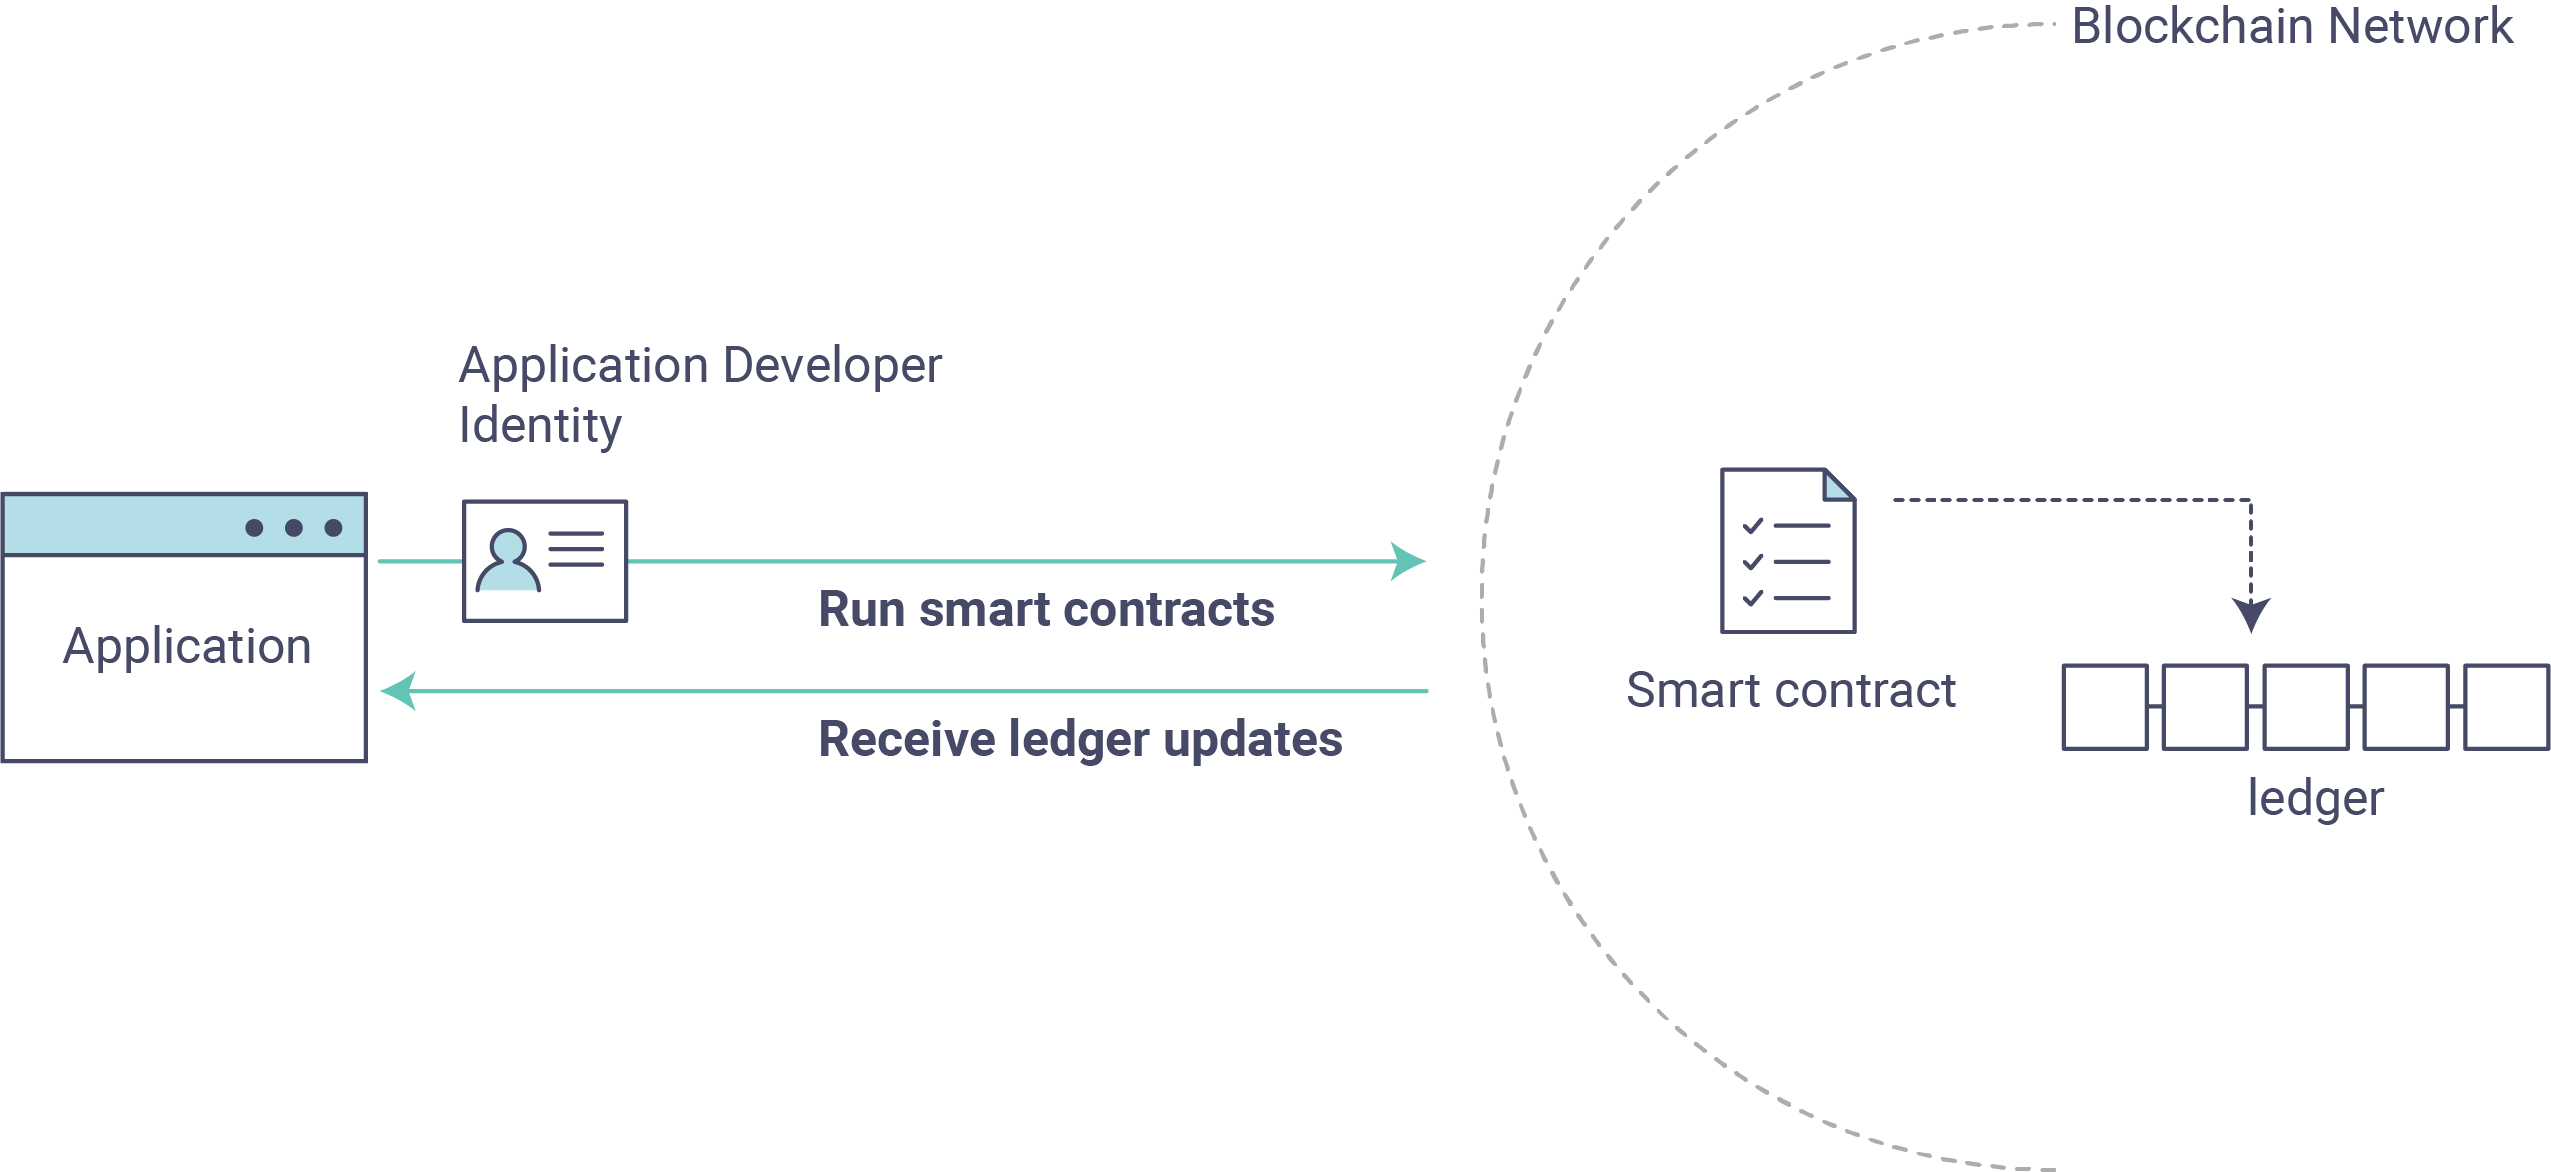
\includegraphics[width=1\linewidth]{imgs/hyperledgerAppOverview.png}
  \caption{\label{fig:appOverview}An Overview of the System Architecture
  (Source:
  \href{http://hyperledger-fabric.readthedocs.io/en/latest/write_first_app.html}{HLF
  Fabric Documentation})} \end{figure}

The application allows for user enrollment to create a new identity in the
network.  When a new user of the application enters the network; the function,
in the smart contract, that initializes the creation of the user and writes the
user to the ledger as a new participating identity is called. Due to the
security mechanisms this specific transaction is automatically signed by the
administrator of the network and is verified by the CA servers.

The smart contract also provides the application with several operations to
manage the identity object as seen on Figure \ref{fig:smartContractOverview}.
These operations form an Application Programming Interface (API) that return a
payload in JSON format with identity information from the network.  This API
allows a query to be made to the network that returns the patients information,
changing incorrect or outdated information or disabling the identity structure
of someone who is not participating in the network actively anymore in order
for that information to be read-only from that point on, for example, with more
available.  Depending on the operation only certain users can access the
information or manipulate the already existing one.  This system architecture
leads to a modular as well as extensible approach regarding the availability of
new operations that become available as soon as new versions of the smart
contract are deployed.  

\begin{figure}[ht] 
  \centering
  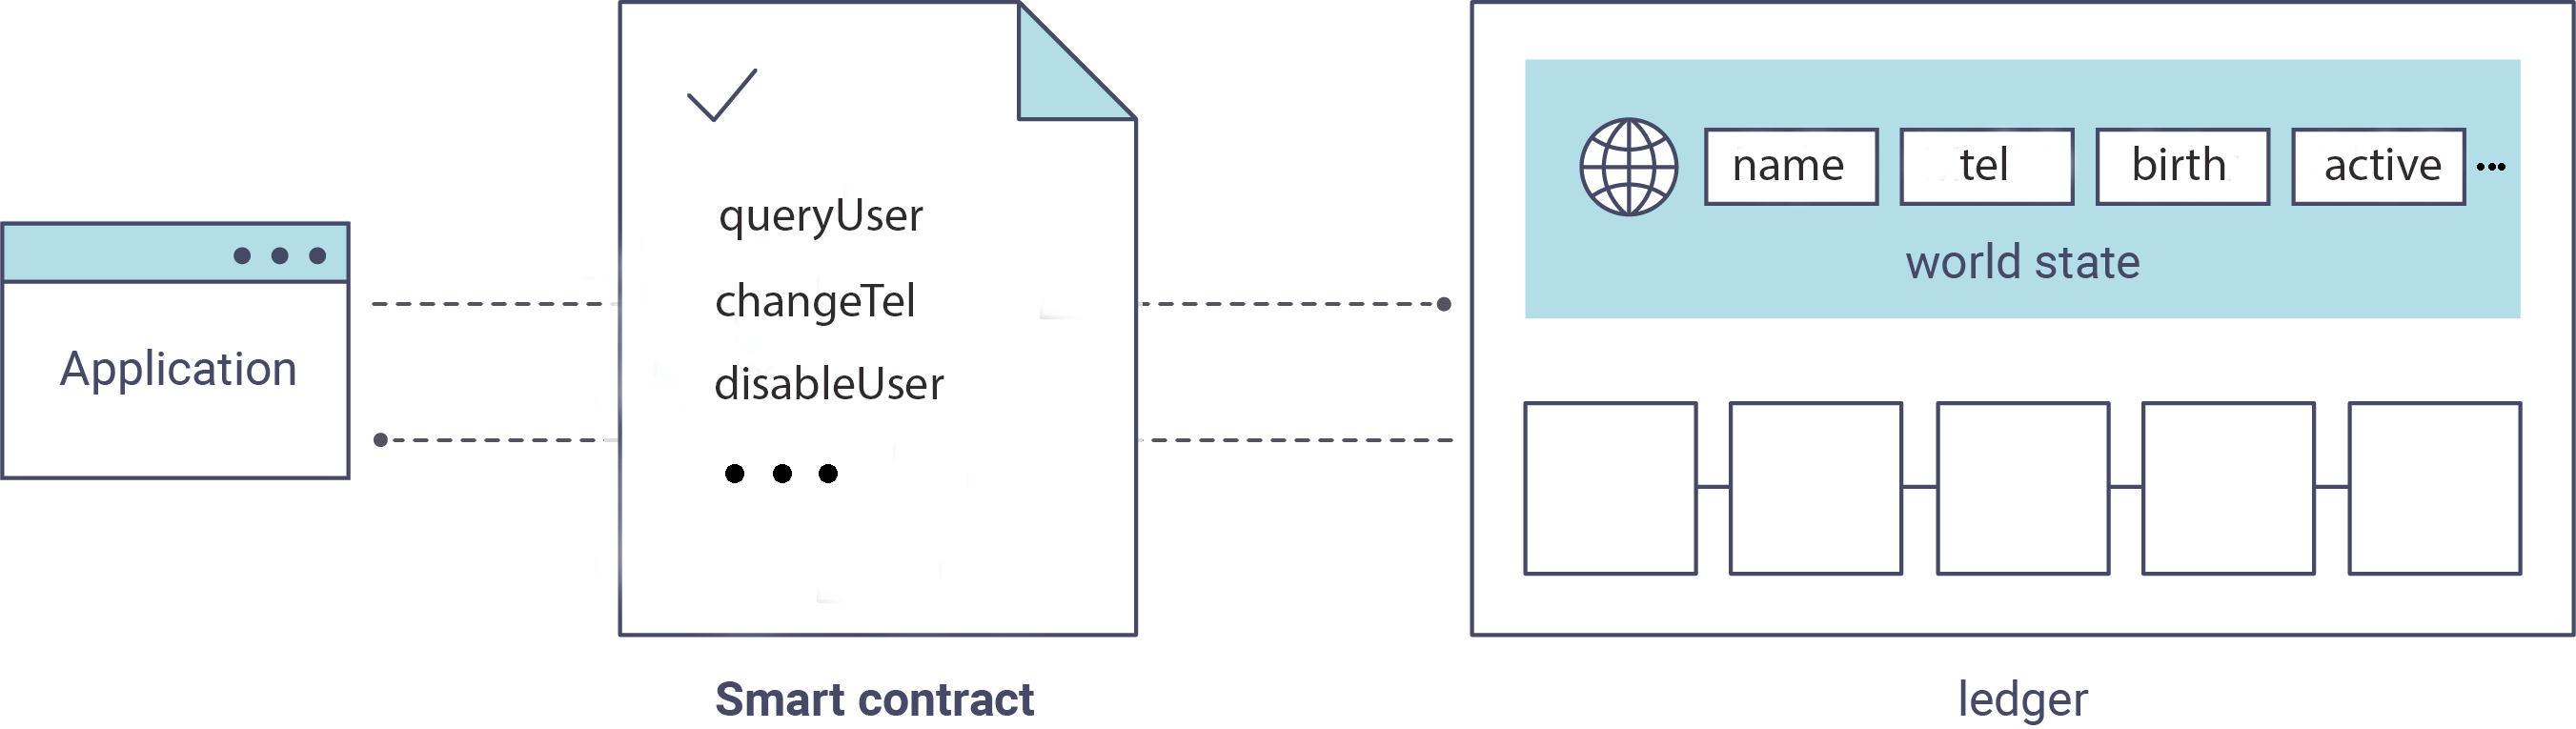
\includegraphics[width=1\linewidth]{imgs/smartContractOverview.png}
  \caption{\label{fig:smartContractOverview}Smart Contract Operations Example
  (Original:
  \href{http://hyperledger-fabric.readthedocs.io/en/latest/write_first_app.html}{HLF
  Fabric Documentation})} 
\end{figure}
